% Figura 7: esquema del ajuste fino de Real-ESRGAN con los datos del proyecto
% Compilar: pdflatex fig07_ajuste_fino.tex
%           pdftoppm -png -r 300 -singlefile fig07_ajuste_fino.pdf ../output/thesis_figures/fig07_ajuste_fino
\documentclass[border=8pt]{standalone}
\usepackage[utf8]{inputenc}
\usepackage[T1]{fontenc}
\usepackage{tikz}
\usetikzlibrary{positioning,arrows.meta,calc}

\begin{document}
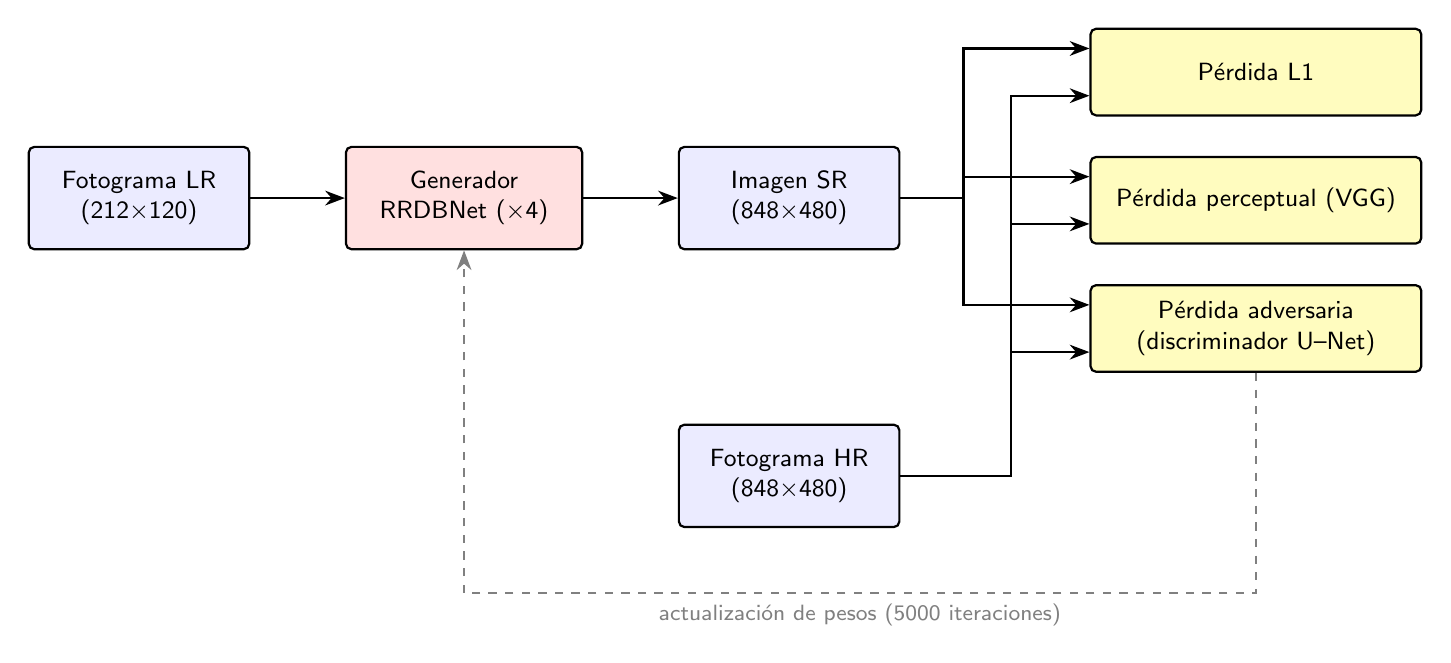
\begin{tikzpicture}[
    font=\sffamily\small,
    dato/.style={draw, rounded corners=2pt, fill=blue!8, minimum width=28mm,
                 minimum height=13mm, align=center, thick},
    red/.style={draw, rounded corners=2pt, fill=red!12, minimum width=30mm,
                minimum height=13mm, align=center, thick},
    perdida/.style={draw, rounded corners=2pt, fill=yellow!25, minimum width=42mm,
                    minimum height=11mm, align=center, thick},
    flecha/.style={-{Stealth[length=2.5mm]}, thick},
    retro/.style={-{Stealth[length=2.5mm]}, thick, dashed, gray}
]

\node[dato]                          (lr)  {Fotograma LR\\(212$\times$120)};
\node[red,  right=12mm of lr]        (gen) {Generador\\RRDBNet ($\times$4)};
\node[dato, right=12mm of gen]       (sr)  {Imagen SR\\(848$\times$480)};

\node[perdida, right=24mm of sr, yshift=16mm] (l1)   {P\'erdida L1};
\node[perdida, below=5mm of l1]               (vgg)  {P\'erdida perceptual (VGG)};
\node[perdida, below=5mm of vgg]              (adv)  {P\'erdida adversaria\\(discriminador U--Net)};

\node[dato, below=22mm of sr] (hr) {Fotograma HR\\(848$\times$480)};

\draw[flecha] (lr) -- (gen);
\draw[flecha] (gen) -- (sr);

% la imagen SR alimenta las tres perdidas por un bus vertical
\coordinate (busSR) at ($(sr.east)+(8mm,0)$);
\draw[thick] (sr.east) -- (busSR);
\draw[flecha] (busSR) |- ([yshift=3mm]l1.west);
\draw[flecha] (busSR) |- ([yshift=3mm]vgg.west);
\draw[flecha] (busSR) |- ([yshift=3mm]adv.west);

% la referencia HR alimenta las mismas perdidas por un segundo bus
\coordinate (busHR) at ($(sr.east)+(14mm,-22mm)$);
\draw[thick] (hr.east) -| (busHR);
\draw[flecha] (busHR) |- ([yshift=-3mm]l1.west);
\draw[flecha] (busHR) |- ([yshift=-3mm]vgg.west);
\draw[flecha] (busHR) |- ([yshift=-3mm]adv.west);

% gradientes de vuelta al generador
\draw[retro] (adv.south) -- ++(0,-28mm) -| (gen.south)
    node[pos=0.25, below, font=\sffamily\footnotesize, text=gray]
    {actualizaci\'on de pesos (5000 iteraciones)};

\end{tikzpicture}
\end{document}
